
% Default to the notebook output style

    


% Inherit from the specified cell style.




    
\documentclass[11pt]{article}

    
    
    \usepackage[T1]{fontenc}
    % Nicer default font (+ math font) than Computer Modern for most use cases
    \usepackage{mathpazo}

    % Basic figure setup, for now with no caption control since it's done
    % automatically by Pandoc (which extracts ![](path) syntax from Markdown).
    \usepackage{graphicx}
    % We will generate all images so they have a width \maxwidth. This means
    % that they will get their normal width if they fit onto the page, but
    % are scaled down if they would overflow the margins.
    \makeatletter
    \def\maxwidth{\ifdim\Gin@nat@width>\linewidth\linewidth
    \else\Gin@nat@width\fi}
    \makeatother
    \let\Oldincludegraphics\includegraphics
    % Set max figure width to be 80% of text width, for now hardcoded.
    \renewcommand{\includegraphics}[1]{\Oldincludegraphics[width=.8\maxwidth]{#1}}
    % Ensure that by default, figures have no caption (until we provide a
    % proper Figure object with a Caption API and a way to capture that
    % in the conversion process - todo).
    \usepackage{caption}
    \DeclareCaptionLabelFormat{nolabel}{}
    \captionsetup{labelformat=nolabel}

    \usepackage{adjustbox} % Used to constrain images to a maximum size 
    \usepackage{xcolor} % Allow colors to be defined
    \usepackage{enumerate} % Needed for markdown enumerations to work
    \usepackage{geometry} % Used to adjust the document margins
    \usepackage{amsmath} % Equations
    \usepackage{amssymb} % Equations
    \usepackage{textcomp} % defines textquotesingle
    % Hack from http://tex.stackexchange.com/a/47451/13684:
    \AtBeginDocument{%
        \def\PYZsq{\textquotesingle}% Upright quotes in Pygmentized code
    }
    \usepackage{upquote} % Upright quotes for verbatim code
    \usepackage{eurosym} % defines \euro
    \usepackage[mathletters]{ucs} % Extended unicode (utf-8) support
    \usepackage[utf8x]{inputenc} % Allow utf-8 characters in the tex document
    \usepackage{fancyvrb} % verbatim replacement that allows latex
    \usepackage{grffile} % extends the file name processing of package graphics 
                         % to support a larger range 
    % The hyperref package gives us a pdf with properly built
    % internal navigation ('pdf bookmarks' for the table of contents,
    % internal cross-reference links, web links for URLs, etc.)
    \usepackage{hyperref}
    \usepackage{longtable} % longtable support required by pandoc >1.10
    \usepackage{booktabs}  % table support for pandoc > 1.12.2
    \usepackage[inline]{enumitem} % IRkernel/repr support (it uses the enumerate* environment)
    \usepackage[normalem]{ulem} % ulem is needed to support strikethroughs (\sout)
                                % normalem makes italics be italics, not underlines
    

    
    
    % Colors for the hyperref package
    \definecolor{urlcolor}{rgb}{0,.145,.698}
    \definecolor{linkcolor}{rgb}{.71,0.21,0.01}
    \definecolor{citecolor}{rgb}{.12,.54,.11}

    % ANSI colors
    \definecolor{ansi-black}{HTML}{3E424D}
    \definecolor{ansi-black-intense}{HTML}{282C36}
    \definecolor{ansi-red}{HTML}{E75C58}
    \definecolor{ansi-red-intense}{HTML}{B22B31}
    \definecolor{ansi-green}{HTML}{00A250}
    \definecolor{ansi-green-intense}{HTML}{007427}
    \definecolor{ansi-yellow}{HTML}{DDB62B}
    \definecolor{ansi-yellow-intense}{HTML}{B27D12}
    \definecolor{ansi-blue}{HTML}{208FFB}
    \definecolor{ansi-blue-intense}{HTML}{0065CA}
    \definecolor{ansi-magenta}{HTML}{D160C4}
    \definecolor{ansi-magenta-intense}{HTML}{A03196}
    \definecolor{ansi-cyan}{HTML}{60C6C8}
    \definecolor{ansi-cyan-intense}{HTML}{258F8F}
    \definecolor{ansi-white}{HTML}{C5C1B4}
    \definecolor{ansi-white-intense}{HTML}{A1A6B2}

    % commands and environments needed by pandoc snippets
    % extracted from the output of `pandoc -s`
    \providecommand{\tightlist}{%
      \setlength{\itemsep}{0pt}\setlength{\parskip}{0pt}}
    \DefineVerbatimEnvironment{Highlighting}{Verbatim}{commandchars=\\\{\}}
    % Add ',fontsize=\small' for more characters per line
    \newenvironment{Shaded}{}{}
    \newcommand{\KeywordTok}[1]{\textcolor[rgb]{0.00,0.44,0.13}{\textbf{{#1}}}}
    \newcommand{\DataTypeTok}[1]{\textcolor[rgb]{0.56,0.13,0.00}{{#1}}}
    \newcommand{\DecValTok}[1]{\textcolor[rgb]{0.25,0.63,0.44}{{#1}}}
    \newcommand{\BaseNTok}[1]{\textcolor[rgb]{0.25,0.63,0.44}{{#1}}}
    \newcommand{\FloatTok}[1]{\textcolor[rgb]{0.25,0.63,0.44}{{#1}}}
    \newcommand{\CharTok}[1]{\textcolor[rgb]{0.25,0.44,0.63}{{#1}}}
    \newcommand{\StringTok}[1]{\textcolor[rgb]{0.25,0.44,0.63}{{#1}}}
    \newcommand{\CommentTok}[1]{\textcolor[rgb]{0.38,0.63,0.69}{\textit{{#1}}}}
    \newcommand{\OtherTok}[1]{\textcolor[rgb]{0.00,0.44,0.13}{{#1}}}
    \newcommand{\AlertTok}[1]{\textcolor[rgb]{1.00,0.00,0.00}{\textbf{{#1}}}}
    \newcommand{\FunctionTok}[1]{\textcolor[rgb]{0.02,0.16,0.49}{{#1}}}
    \newcommand{\RegionMarkerTok}[1]{{#1}}
    \newcommand{\ErrorTok}[1]{\textcolor[rgb]{1.00,0.00,0.00}{\textbf{{#1}}}}
    \newcommand{\NormalTok}[1]{{#1}}
    
    % Additional commands for more recent versions of Pandoc
    \newcommand{\ConstantTok}[1]{\textcolor[rgb]{0.53,0.00,0.00}{{#1}}}
    \newcommand{\SpecialCharTok}[1]{\textcolor[rgb]{0.25,0.44,0.63}{{#1}}}
    \newcommand{\VerbatimStringTok}[1]{\textcolor[rgb]{0.25,0.44,0.63}{{#1}}}
    \newcommand{\SpecialStringTok}[1]{\textcolor[rgb]{0.73,0.40,0.53}{{#1}}}
    \newcommand{\ImportTok}[1]{{#1}}
    \newcommand{\DocumentationTok}[1]{\textcolor[rgb]{0.73,0.13,0.13}{\textit{{#1}}}}
    \newcommand{\AnnotationTok}[1]{\textcolor[rgb]{0.38,0.63,0.69}{\textbf{\textit{{#1}}}}}
    \newcommand{\CommentVarTok}[1]{\textcolor[rgb]{0.38,0.63,0.69}{\textbf{\textit{{#1}}}}}
    \newcommand{\VariableTok}[1]{\textcolor[rgb]{0.10,0.09,0.49}{{#1}}}
    \newcommand{\ControlFlowTok}[1]{\textcolor[rgb]{0.00,0.44,0.13}{\textbf{{#1}}}}
    \newcommand{\OperatorTok}[1]{\textcolor[rgb]{0.40,0.40,0.40}{{#1}}}
    \newcommand{\BuiltInTok}[1]{{#1}}
    \newcommand{\ExtensionTok}[1]{{#1}}
    \newcommand{\PreprocessorTok}[1]{\textcolor[rgb]{0.74,0.48,0.00}{{#1}}}
    \newcommand{\AttributeTok}[1]{\textcolor[rgb]{0.49,0.56,0.16}{{#1}}}
    \newcommand{\InformationTok}[1]{\textcolor[rgb]{0.38,0.63,0.69}{\textbf{\textit{{#1}}}}}
    \newcommand{\WarningTok}[1]{\textcolor[rgb]{0.38,0.63,0.69}{\textbf{\textit{{#1}}}}}
    
    
    % Define a nice break command that doesn't care if a line doesn't already
    % exist.
    \def\br{\hspace*{\fill} \\* }
    % Math Jax compatability definitions
    \def\gt{>}
    \def\lt{<}
    % Document parameters
    \title{Problem set 1: Math for Machine
Learning}
    \author{Jiarong Ye}
    
    

    % Pygments definitions
    
\makeatletter
\def\PY@reset{\let\PY@it=\relax \let\PY@bf=\relax%
    \let\PY@ul=\relax \let\PY@tc=\relax%
    \let\PY@bc=\relax \let\PY@ff=\relax}
\def\PY@tok#1{\csname PY@tok@#1\endcsname}
\def\PY@toks#1+{\ifx\relax#1\empty\else%
    \PY@tok{#1}\expandafter\PY@toks\fi}
\def\PY@do#1{\PY@bc{\PY@tc{\PY@ul{%
    \PY@it{\PY@bf{\PY@ff{#1}}}}}}}
\def\PY#1#2{\PY@reset\PY@toks#1+\relax+\PY@do{#2}}

\expandafter\def\csname PY@tok@dl\endcsname{\def\PY@tc##1{\textcolor[rgb]{0.73,0.13,0.13}{##1}}}
\expandafter\def\csname PY@tok@ni\endcsname{\let\PY@bf=\textbf\def\PY@tc##1{\textcolor[rgb]{0.60,0.60,0.60}{##1}}}
\expandafter\def\csname PY@tok@s\endcsname{\def\PY@tc##1{\textcolor[rgb]{0.73,0.13,0.13}{##1}}}
\expandafter\def\csname PY@tok@kr\endcsname{\let\PY@bf=\textbf\def\PY@tc##1{\textcolor[rgb]{0.00,0.50,0.00}{##1}}}
\expandafter\def\csname PY@tok@no\endcsname{\def\PY@tc##1{\textcolor[rgb]{0.53,0.00,0.00}{##1}}}
\expandafter\def\csname PY@tok@go\endcsname{\def\PY@tc##1{\textcolor[rgb]{0.53,0.53,0.53}{##1}}}
\expandafter\def\csname PY@tok@sd\endcsname{\let\PY@it=\textit\def\PY@tc##1{\textcolor[rgb]{0.73,0.13,0.13}{##1}}}
\expandafter\def\csname PY@tok@mo\endcsname{\def\PY@tc##1{\textcolor[rgb]{0.40,0.40,0.40}{##1}}}
\expandafter\def\csname PY@tok@nd\endcsname{\def\PY@tc##1{\textcolor[rgb]{0.67,0.13,1.00}{##1}}}
\expandafter\def\csname PY@tok@vm\endcsname{\def\PY@tc##1{\textcolor[rgb]{0.10,0.09,0.49}{##1}}}
\expandafter\def\csname PY@tok@mh\endcsname{\def\PY@tc##1{\textcolor[rgb]{0.40,0.40,0.40}{##1}}}
\expandafter\def\csname PY@tok@cs\endcsname{\let\PY@it=\textit\def\PY@tc##1{\textcolor[rgb]{0.25,0.50,0.50}{##1}}}
\expandafter\def\csname PY@tok@ow\endcsname{\let\PY@bf=\textbf\def\PY@tc##1{\textcolor[rgb]{0.67,0.13,1.00}{##1}}}
\expandafter\def\csname PY@tok@nt\endcsname{\let\PY@bf=\textbf\def\PY@tc##1{\textcolor[rgb]{0.00,0.50,0.00}{##1}}}
\expandafter\def\csname PY@tok@k\endcsname{\let\PY@bf=\textbf\def\PY@tc##1{\textcolor[rgb]{0.00,0.50,0.00}{##1}}}
\expandafter\def\csname PY@tok@ge\endcsname{\let\PY@it=\textit}
\expandafter\def\csname PY@tok@sb\endcsname{\def\PY@tc##1{\textcolor[rgb]{0.73,0.13,0.13}{##1}}}
\expandafter\def\csname PY@tok@err\endcsname{\def\PY@bc##1{\setlength{\fboxsep}{0pt}\fcolorbox[rgb]{1.00,0.00,0.00}{1,1,1}{\strut ##1}}}
\expandafter\def\csname PY@tok@bp\endcsname{\def\PY@tc##1{\textcolor[rgb]{0.00,0.50,0.00}{##1}}}
\expandafter\def\csname PY@tok@gt\endcsname{\def\PY@tc##1{\textcolor[rgb]{0.00,0.27,0.87}{##1}}}
\expandafter\def\csname PY@tok@gp\endcsname{\let\PY@bf=\textbf\def\PY@tc##1{\textcolor[rgb]{0.00,0.00,0.50}{##1}}}
\expandafter\def\csname PY@tok@nl\endcsname{\def\PY@tc##1{\textcolor[rgb]{0.63,0.63,0.00}{##1}}}
\expandafter\def\csname PY@tok@m\endcsname{\def\PY@tc##1{\textcolor[rgb]{0.40,0.40,0.40}{##1}}}
\expandafter\def\csname PY@tok@kd\endcsname{\let\PY@bf=\textbf\def\PY@tc##1{\textcolor[rgb]{0.00,0.50,0.00}{##1}}}
\expandafter\def\csname PY@tok@sa\endcsname{\def\PY@tc##1{\textcolor[rgb]{0.73,0.13,0.13}{##1}}}
\expandafter\def\csname PY@tok@gi\endcsname{\def\PY@tc##1{\textcolor[rgb]{0.00,0.63,0.00}{##1}}}
\expandafter\def\csname PY@tok@gs\endcsname{\let\PY@bf=\textbf}
\expandafter\def\csname PY@tok@mb\endcsname{\def\PY@tc##1{\textcolor[rgb]{0.40,0.40,0.40}{##1}}}
\expandafter\def\csname PY@tok@cp\endcsname{\def\PY@tc##1{\textcolor[rgb]{0.74,0.48,0.00}{##1}}}
\expandafter\def\csname PY@tok@nv\endcsname{\def\PY@tc##1{\textcolor[rgb]{0.10,0.09,0.49}{##1}}}
\expandafter\def\csname PY@tok@gd\endcsname{\def\PY@tc##1{\textcolor[rgb]{0.63,0.00,0.00}{##1}}}
\expandafter\def\csname PY@tok@gh\endcsname{\let\PY@bf=\textbf\def\PY@tc##1{\textcolor[rgb]{0.00,0.00,0.50}{##1}}}
\expandafter\def\csname PY@tok@w\endcsname{\def\PY@tc##1{\textcolor[rgb]{0.73,0.73,0.73}{##1}}}
\expandafter\def\csname PY@tok@kn\endcsname{\let\PY@bf=\textbf\def\PY@tc##1{\textcolor[rgb]{0.00,0.50,0.00}{##1}}}
\expandafter\def\csname PY@tok@kc\endcsname{\let\PY@bf=\textbf\def\PY@tc##1{\textcolor[rgb]{0.00,0.50,0.00}{##1}}}
\expandafter\def\csname PY@tok@sh\endcsname{\def\PY@tc##1{\textcolor[rgb]{0.73,0.13,0.13}{##1}}}
\expandafter\def\csname PY@tok@mi\endcsname{\def\PY@tc##1{\textcolor[rgb]{0.40,0.40,0.40}{##1}}}
\expandafter\def\csname PY@tok@ss\endcsname{\def\PY@tc##1{\textcolor[rgb]{0.10,0.09,0.49}{##1}}}
\expandafter\def\csname PY@tok@o\endcsname{\def\PY@tc##1{\textcolor[rgb]{0.40,0.40,0.40}{##1}}}
\expandafter\def\csname PY@tok@kt\endcsname{\def\PY@tc##1{\textcolor[rgb]{0.69,0.00,0.25}{##1}}}
\expandafter\def\csname PY@tok@mf\endcsname{\def\PY@tc##1{\textcolor[rgb]{0.40,0.40,0.40}{##1}}}
\expandafter\def\csname PY@tok@vi\endcsname{\def\PY@tc##1{\textcolor[rgb]{0.10,0.09,0.49}{##1}}}
\expandafter\def\csname PY@tok@sr\endcsname{\def\PY@tc##1{\textcolor[rgb]{0.73,0.40,0.53}{##1}}}
\expandafter\def\csname PY@tok@na\endcsname{\def\PY@tc##1{\textcolor[rgb]{0.49,0.56,0.16}{##1}}}
\expandafter\def\csname PY@tok@cpf\endcsname{\let\PY@it=\textit\def\PY@tc##1{\textcolor[rgb]{0.25,0.50,0.50}{##1}}}
\expandafter\def\csname PY@tok@c1\endcsname{\let\PY@it=\textit\def\PY@tc##1{\textcolor[rgb]{0.25,0.50,0.50}{##1}}}
\expandafter\def\csname PY@tok@ch\endcsname{\let\PY@it=\textit\def\PY@tc##1{\textcolor[rgb]{0.25,0.50,0.50}{##1}}}
\expandafter\def\csname PY@tok@nc\endcsname{\let\PY@bf=\textbf\def\PY@tc##1{\textcolor[rgb]{0.00,0.00,1.00}{##1}}}
\expandafter\def\csname PY@tok@s1\endcsname{\def\PY@tc##1{\textcolor[rgb]{0.73,0.13,0.13}{##1}}}
\expandafter\def\csname PY@tok@nb\endcsname{\def\PY@tc##1{\textcolor[rgb]{0.00,0.50,0.00}{##1}}}
\expandafter\def\csname PY@tok@il\endcsname{\def\PY@tc##1{\textcolor[rgb]{0.40,0.40,0.40}{##1}}}
\expandafter\def\csname PY@tok@vg\endcsname{\def\PY@tc##1{\textcolor[rgb]{0.10,0.09,0.49}{##1}}}
\expandafter\def\csname PY@tok@gu\endcsname{\let\PY@bf=\textbf\def\PY@tc##1{\textcolor[rgb]{0.50,0.00,0.50}{##1}}}
\expandafter\def\csname PY@tok@vc\endcsname{\def\PY@tc##1{\textcolor[rgb]{0.10,0.09,0.49}{##1}}}
\expandafter\def\csname PY@tok@se\endcsname{\let\PY@bf=\textbf\def\PY@tc##1{\textcolor[rgb]{0.73,0.40,0.13}{##1}}}
\expandafter\def\csname PY@tok@cm\endcsname{\let\PY@it=\textit\def\PY@tc##1{\textcolor[rgb]{0.25,0.50,0.50}{##1}}}
\expandafter\def\csname PY@tok@nn\endcsname{\let\PY@bf=\textbf\def\PY@tc##1{\textcolor[rgb]{0.00,0.00,1.00}{##1}}}
\expandafter\def\csname PY@tok@ne\endcsname{\let\PY@bf=\textbf\def\PY@tc##1{\textcolor[rgb]{0.82,0.25,0.23}{##1}}}
\expandafter\def\csname PY@tok@kp\endcsname{\def\PY@tc##1{\textcolor[rgb]{0.00,0.50,0.00}{##1}}}
\expandafter\def\csname PY@tok@si\endcsname{\let\PY@bf=\textbf\def\PY@tc##1{\textcolor[rgb]{0.73,0.40,0.53}{##1}}}
\expandafter\def\csname PY@tok@s2\endcsname{\def\PY@tc##1{\textcolor[rgb]{0.73,0.13,0.13}{##1}}}
\expandafter\def\csname PY@tok@fm\endcsname{\def\PY@tc##1{\textcolor[rgb]{0.00,0.00,1.00}{##1}}}
\expandafter\def\csname PY@tok@sc\endcsname{\def\PY@tc##1{\textcolor[rgb]{0.73,0.13,0.13}{##1}}}
\expandafter\def\csname PY@tok@sx\endcsname{\def\PY@tc##1{\textcolor[rgb]{0.00,0.50,0.00}{##1}}}
\expandafter\def\csname PY@tok@c\endcsname{\let\PY@it=\textit\def\PY@tc##1{\textcolor[rgb]{0.25,0.50,0.50}{##1}}}
\expandafter\def\csname PY@tok@gr\endcsname{\def\PY@tc##1{\textcolor[rgb]{1.00,0.00,0.00}{##1}}}
\expandafter\def\csname PY@tok@nf\endcsname{\def\PY@tc##1{\textcolor[rgb]{0.00,0.00,1.00}{##1}}}

\def\PYZbs{\char`\\}
\def\PYZus{\char`\_}
\def\PYZob{\char`\{}
\def\PYZcb{\char`\}}
\def\PYZca{\char`\^}
\def\PYZam{\char`\&}
\def\PYZlt{\char`\<}
\def\PYZgt{\char`\>}
\def\PYZsh{\char`\#}
\def\PYZpc{\char`\%}
\def\PYZdl{\char`\$}
\def\PYZhy{\char`\-}
\def\PYZsq{\char`\'}
\def\PYZdq{\char`\"}
\def\PYZti{\char`\~}
% for compatibility with earlier versions
\def\PYZat{@}
\def\PYZlb{[}
\def\PYZrb{]}
\makeatother


    % Exact colors from NB
    \definecolor{incolor}{rgb}{0.0, 0.0, 0.5}
    \definecolor{outcolor}{rgb}{0.545, 0.0, 0.0}



    
    % Prevent overflowing lines due to hard-to-break entities
    \sloppy 
    % Setup hyperref package
    \hypersetup{
      breaklinks=true,  % so long urls are correctly broken across lines
      colorlinks=true,
      urlcolor=urlcolor,
      linkcolor=linkcolor,
      citecolor=citecolor,
      }
    % Slightly bigger margins than the latex defaults
    
    \geometry{verbose,tmargin=1in,bmargin=1in,lmargin=1in,rmargin=1in}
    
    

    \begin{document}
    
    
    \maketitle
    
    


    \subsubsection*{Q1}\label{q1}

    1.(20 pts.) Let X = {[}2, −2{]} be a vector.

\begin{enumerate}
\def\labelenumi{(\alph{enumi})}
\tightlist
\item
  Plot the vector in a 2-dimensional Euclidean space
\end{enumerate}

    \begin{Verbatim}[commandchars=\\\{\}]
{\color{incolor}In [{\color{incolor}1}]:} \PY{k+kn}{import} \PY{n+nn}{numpy} \PY{k}{as} \PY{n+nn}{np}
        \PY{k+kn}{import} \PY{n+nn}{matplotlib}\PY{n+nn}{.}\PY{n+nn}{pyplot} \PY{k}{as} \PY{n+nn}{plt}
        \PY{o}{\PYZpc{}}\PY{k}{matplotlib} inline
        
        \PY{k}{def} \PY{n+nf}{draw\PYZus{}vector}\PY{p}{(}\PY{n}{x}\PY{p}{)}\PY{p}{:}
            \PY{n}{plt}\PY{o}{.}\PY{n}{figure}\PY{p}{(}\PY{n}{figsize}\PY{o}{=}\PY{p}{(}\PY{l+m+mi}{8}\PY{p}{,} \PY{l+m+mi}{8}\PY{p}{)}\PY{p}{)}
            \PY{k}{for} \PY{n}{i} \PY{o+ow}{in} \PY{n}{x}\PY{p}{:}
                \PY{n}{X}\PY{p}{,} \PY{n}{Y}\PY{p}{,} \PY{n}{U}\PY{p}{,} \PY{n}{V} \PY{o}{=} \PY{n+nb}{zip}\PY{p}{(}\PY{o}{*}\PY{n}{np}\PY{o}{.}\PY{n}{array}\PY{p}{(}\PY{n}{x}\PY{p}{)}\PY{p}{)}
                \PY{n}{ax} \PY{o}{=} \PY{n}{plt}\PY{o}{.}\PY{n}{gca}\PY{p}{(}\PY{p}{)}
                \PY{n}{ax}\PY{o}{.}\PY{n}{quiver}\PY{p}{(}\PY{n}{X}\PY{p}{,} \PY{n}{Y}\PY{p}{,} \PY{n}{U}\PY{p}{,} \PY{n}{V}\PY{p}{,} \PY{n}{angles}\PY{o}{=}\PY{l+s+s1}{\PYZsq{}}\PY{l+s+s1}{xy}\PY{l+s+s1}{\PYZsq{}}\PY{p}{,} \PY{n}{scale\PYZus{}units}\PY{o}{=}\PY{l+s+s1}{\PYZsq{}}\PY{l+s+s1}{xy}\PY{l+s+s1}{\PYZsq{}}\PY{p}{,} \PY{n}{scale}\PY{o}{=}\PY{l+m+mi}{1}\PY{p}{)}
                \PY{n}{ax}\PY{o}{.}\PY{n}{annotate}\PY{p}{(}\PY{l+s+s1}{\PYZsq{}}\PY{l+s+s1}{X = [}\PY{l+s+si}{\PYZob{}\PYZcb{}}\PY{l+s+s1}{, }\PY{l+s+si}{\PYZob{}\PYZcb{}}\PY{l+s+s1}{] }\PY{l+s+s1}{\PYZsq{}}\PY{o}{.}\PY{n}{format}\PY{p}{(}\PY{n}{i}\PY{p}{[}\PY{l+m+mi}{2}\PY{p}{]}\PY{p}{,} \PY{n}{i}\PY{p}{[}\PY{l+m+mi}{3}\PY{p}{]}\PY{p}{)}\PY{p}{,} \PY{n}{xy}\PY{o}{=}\PY{p}{(}\PY{n}{i}\PY{p}{[}\PY{l+m+mi}{2}\PY{p}{]}\PY{o}{\PYZhy{}}\PY{l+m+mi}{1}\PY{p}{,} \PY{n}{i}\PY{p}{[}\PY{l+m+mi}{3}\PY{p}{]}\PY{o}{\PYZhy{}}\PY{l+m+mf}{0.2}\PY{p}{)}\PY{p}{)}
            \PY{n}{ax}\PY{o}{.}\PY{n}{set\PYZus{}xlim}\PY{p}{(}\PY{p}{[}\PY{o}{\PYZhy{}}\PY{l+m+mf}{2.5}\PY{p}{,} \PY{l+m+mf}{2.5}\PY{p}{]}\PY{p}{)}
            \PY{n}{ax}\PY{o}{.}\PY{n}{set\PYZus{}ylim}\PY{p}{(}\PY{p}{[}\PY{o}{\PYZhy{}}\PY{l+m+mf}{2.5}\PY{p}{,} \PY{l+m+mf}{2.5}\PY{p}{]}\PY{p}{)}
            \PY{n}{plt}\PY{o}{.}\PY{n}{grid}\PY{p}{(}\PY{k+kc}{True}\PY{p}{)}
            \PY{n}{plt}\PY{o}{.}\PY{n}{draw}\PY{p}{(}\PY{p}{)}
            \PY{n}{plt}\PY{o}{.}\PY{n}{show}\PY{p}{(}\PY{p}{)}
\end{Verbatim}


    \begin{Verbatim}[commandchars=\\\{\}]
{\color{incolor}In [{\color{incolor}2}]:} \PY{n}{draw\PYZus{}vector}\PY{p}{(}\PY{p}{[}\PY{p}{[}\PY{l+m+mi}{0}\PY{p}{,}\PY{l+m+mi}{0}\PY{p}{,}\PY{l+m+mi}{2}\PY{p}{,}\PY{o}{\PYZhy{}}\PY{l+m+mi}{2}\PY{p}{]}\PY{p}{]}\PY{p}{)}
\end{Verbatim}


    \begin{center}
    \adjustimage{max size={0.4\linewidth}{0.4\paperheight}}{output_4_0.png}
    \end{center}
    { \hspace*{\fill} \\}
    
    \begin{enumerate}
\def\labelenumi{(\alph{enumi})}
\setcounter{enumi}{1}
\tightlist
\item
  Compute the Euclidian norm of the vector X.
\end{enumerate}

The general case of Euclidian norm of a vector:
\[{\displaystyle \left\|{\boldsymbol {x}}\right\|_{2}={\sqrt {x_{1}^{2}+\cdots +x_{n}^{2}}}}\]

Thus, the Euclidian norm of the vector X is:

\[\left\| x \right\|_2 = \sqrt{2^2 + (-2)^2} = 2 \sqrt{2}\]

    \begin{enumerate}
\def\labelenumi{(\alph{enumi})}
\setcounter{enumi}{2}
\tightlist
\item
  Normalize the vector X to obtain a vector of unit length
\end{enumerate}

\[\text{normalized X } = \frac{X}{\left\| x \right\|_2}  = \left [\frac{2}{\left\| x \right\|_2}, \frac{-2}{\left\| x \right\|_2}\right ] = \left [\frac{2}{2\sqrt{2}}, \frac{-2}{2\sqrt{2}}\right ] = \left [\frac{\sqrt{2}}{2}, -\frac{\sqrt{2}}{2} \right ]\]

check the answer:

\[\text{ length of normalized X } = \sqrt{\left (\frac{\sqrt{2}}{2} \right )^2 + \left (-\frac{\sqrt{2}}{2} \right )^2} = \sqrt{\frac{1}{2} + \frac{1}{2}} = 1 \]

\[\text {so the normalized vector X is unit length, the answer is checked.} \]

    \begin{enumerate}
\def\labelenumi{(\alph{enumi})}
\setcounter{enumi}{3}
\tightlist
\item
  Compute the vector that is normal to X.
\end{enumerate}

Since the vector \(X = [2, -2]\) in a 2-dimensional Euclidean space
could be written as a line:

\[x+y = 0\]

the normal vector of a 2-dimensional line will have the direction vector
of an orthogonal line to it, and the perpendicular vector is (1,1) in
this case.

So the vector that is normal to X is \([1, 1]\)

    \begin{Verbatim}[commandchars=\\\{\}]
{\color{incolor}In [{\color{incolor}3}]:} \PY{c+c1}{\PYZsh{} check the graph:}
        \PY{n}{draw\PYZus{}vector}\PY{p}{(}\PY{p}{[}\PY{p}{[}\PY{l+m+mi}{0}\PY{p}{,}\PY{l+m+mi}{0}\PY{p}{,}\PY{l+m+mi}{2}\PY{p}{,}\PY{o}{\PYZhy{}}\PY{l+m+mi}{2}\PY{p}{]}\PY{p}{,} \PY{p}{[}\PY{l+m+mi}{0}\PY{p}{,}\PY{l+m+mi}{0}\PY{p}{,}\PY{l+m+mi}{1}\PY{p}{,}\PY{l+m+mi}{1}\PY{p}{]}\PY{p}{]}\PY{p}{)}
\end{Verbatim}


    \begin{center}
    \adjustimage{max size={0.4\linewidth}{0.4\paperheight}}{output_8_0.png}
    \end{center}
    { \hspace*{\fill} \\}
    
    \begin{enumerate}
\def\labelenumi{(\alph{enumi})}
\setcounter{enumi}{4}
\tightlist
\item
  Compute the transpose of the vector X.
\end{enumerate}

The transpose vector of X is:

\[X^T = \begin{bmatrix} 2
\\ -2
\end{bmatrix}\]

    \subsubsection*{Q2}\label{q2}

    2.(20 pts.) Joe takes a lab test and the result comes back positive. The
test returns a correct positive result in only 98\% of the cases in
which the disease is actually present, and a correct negative result in
only 97\% of the cases in which the disease is not present. Furthermore,
.008 of the entire population have this cancer. Does Joe have cancer?
Justify your answer.

    \[P(cancer) = 0.008\] \[P(no \: cancer) = 0.992\]

\[P(positive \mid cancer) = 0.98\] \[P(negative \mid cancer) = 0.02\]

\[P(negative \mid no \: cancer) = 0.97\]
\[P(positive \mid no \: cancer) = 0.03\]

Since the result of Joe's test comes back as positive:

Thus

\begin{align}P(cancer \mid positive) &= \frac{P(positive, cancer)}{P(positive)} \\
&= \frac{P(positive\mid cancer) P(cancer)}{P(positive \mid cancer) P(cancer) + P(positive \mid no \: cancer)P(no \: cancer)}
\end{align}

And since:

\[P(positive\mid cancer) P(cancer) = (0.98)(0.008)=0.00784\]

\begin{align}P(positive \mid cancer) P(cancer) + P(positive \mid no \: cancer)P(no \: cancer)\\
= (0.98)(0.008)+(0.03)(0.992)= 0.0376
\end{align}

\begin{align}P(cancer \mid positive) &= \frac{P(positive, cancer)}{P(positive)} \\
&= \frac{P(positive\mid cancer) P(cancer)}{P(positive \mid cancer) P(cancer) + P(positive \mid no \: cancer)P(no \: cancer)} \\
&=\frac{0.00784}{0.0376} \\
&= 0.2085
\end{align}

With Joe's test result being positive, there's approximately 20.85\%
chance that Joe have cancer, so he most likely does not have cancer.

    \subsubsection*{Q3}\label{q3}

    3.(20 pts.) Consider the function \(f(x, y) = x^2 + xy + y^2\).

    \begin{enumerate}
\def\labelenumi{(\alph{enumi})}
\tightlist
\item
  Compute the first order partial derivatives \(\partial fx\) and
  \(\partial fy\)
\end{enumerate}

    \[\partial fx = \frac{\partial (x^2 + xy + y^2)}{\partial x} = 2x+y\]

\[\partial fy = \frac{\partial (x^2 + xy + y^2)}{\partial y} = 2y+x\]

    \begin{enumerate}
\def\labelenumi{(\alph{enumi})}
\setcounter{enumi}{1}
\tightlist
\item
  Compute the Hessian (matrix of second order partial derivatives) of f.
\end{enumerate}

    \begin{align} H=
\begin{bmatrix} \frac{\partial^2 f}{\partial x^2}
 & \frac{\partial^2 f}{\partial x \partial y}\\ 
 \frac{\partial^2 f}{\partial y \partial x} 
 & \frac{\partial^2 f}{\partial y^2}
\end{bmatrix}
\end{align}

\[\frac{\partial^2 f}{\partial x^2} = 2\]

\[\frac{\partial^2 f}{\partial x \partial y} = 1\]

\[\frac{\partial^2 f}{\partial y \partial x} = 1\]

\[\frac{\partial^2 f}{\partial y^2} = 2\]

\begin{align} H=
\begin{bmatrix} \frac{\partial^2 f}{\partial x^2}
 & \frac{\partial^2 f}{\partial x \partial y}\\ 
 \frac{\partial^2 f}{\partial y \partial x} 
 & \frac{\partial^2 f}{\partial y^2}
\end{bmatrix} = 
\begin{bmatrix} 2
 & 1\\ 
1 
 & 2
\end{bmatrix}
\end{align}

    \begin{enumerate}
\def\labelenumi{(\alph{enumi})}
\setcounter{enumi}{2}
\tightlist
\item
  Is f(x, y) a convex function of x and y? Justify your answer.
\end{enumerate}

    \begin{figure}[htbp]
\centering
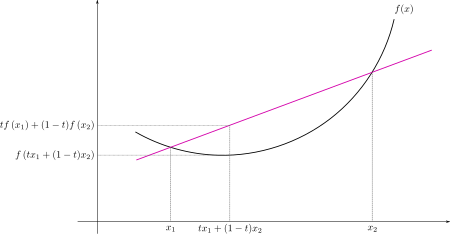
\includegraphics{../../images/convex.png}
\caption{}
\end{figure}

As shown in the graph, a function \(f(x)\) is considered as convex on an
interval \([a,b]\) if for any two points \(x_1\) and \(x_2\) in
\([a,b]\) and any \(\lambda\) where \(0<\lambda<1\)

\[ f[\lambda x_1+(1-\lambda)x_2] \le \lambda f(x_1)+(1-\lambda)f(x_2) \]

And a convenient test for convexity is to calculate its second
derivative since a twice differentiable function of one variable is
convex on an interval if and only if its second derivative is
non-negative.

\begin{itemize}
\item
  for \(x\) , \(f(x) = x^2+xy +y^2\),
  \[\frac{\partial^2 f}{\partial x^2} = 2 \ge 0\] so \(f(x,y)\) is a
  convex function of \(x\)
\item
  for \(y\) , \(f(y) = y^2+yx +x^2\),
  \[\frac{\partial^2 f}{\partial y^2} = 2 \ge 0\] so \(f(x,y)\) is a
  convex function of \(y\)
\end{itemize}

In conclusion, \(f(x, y)\) a convex function of \(x\) and \(y\)

    \begin{enumerate}
\def\labelenumi{(\alph{enumi})}
\setcounter{enumi}{3}
\tightlist
\item
  Compute the values of \(x\) and \(y\) at which \(f(x, y)\) is
  minimized.
\end{enumerate}

    Since we already know from part (c) that \(f(x,y) = x^2+xy+y^2\) is
convex for both \(x\) and \(y\), so when \(f(x, y)\) is minimized,
there's only one global minimum value exists (no local extremes).

Thus, the requirement for \(\min f(x, y)\) is:

\begin{align} \triangledown f =
\begin{bmatrix} \frac{\partial f}{\partial x} 
\\  \frac{\partial f}{\partial y } 
\end{bmatrix} = 
\begin{bmatrix} 2x+y
\\  2y+x
\end{bmatrix} = 
\begin{bmatrix} 0
\\  0
\end{bmatrix} 
\end{align}

So:

\[\left\{\begin{matrix} x=0
\\ y=0
\end{matrix}\right.\]

check the graph of \(f(x,y)\):

    \begin{Verbatim}[commandchars=\\\{\}]
{\color{incolor}In [{\color{incolor}4}]:} \PY{k+kn}{from} \PY{n+nn}{numpy} \PY{k}{import} \PY{n}{exp}\PY{p}{,}\PY{n}{arange}
        \PY{k+kn}{from} \PY{n+nn}{pylab} \PY{k}{import} \PY{n}{meshgrid}\PY{p}{,}\PY{n}{cm}\PY{p}{,}\PY{n}{imshow}\PY{p}{,}\PY{n}{contour}\PY{p}{,}\PY{n}{clabel}\PY{p}{,}\PY{n}{colorbar}\PY{p}{,}\PY{n}{axis}\PY{p}{,}\PY{n}{title}\PY{p}{,}\PY{n}{show}
        \PY{k+kn}{from} \PY{n+nn}{mpl\PYZus{}toolkits}\PY{n+nn}{.}\PY{n+nn}{mplot3d} \PY{k}{import} \PY{n}{Axes3D}
        \PY{k+kn}{from} \PY{n+nn}{matplotlib} \PY{k}{import} \PY{n}{cm}
        \PY{k+kn}{from} \PY{n+nn}{matplotlib}\PY{n+nn}{.}\PY{n+nn}{ticker} \PY{k}{import} \PY{n}{LinearLocator}\PY{p}{,} \PY{n}{FormatStrFormatter}
        \PY{k+kn}{import} \PY{n+nn}{matplotlib}\PY{n+nn}{.}\PY{n+nn}{pyplot} \PY{k}{as} \PY{n+nn}{plt}
        
        \PY{k}{def} \PY{n+nf}{plot\PYZus{}func}\PY{p}{(}\PY{n}{angle\PYZus{}up}\PY{p}{,} \PY{n}{angle\PYZus{}side}\PY{p}{)}\PY{p}{:}
            \PY{n}{x} \PY{o}{=} \PY{n}{arange}\PY{p}{(}\PY{o}{\PYZhy{}}\PY{l+m+mf}{5.0}\PY{p}{,}\PY{l+m+mf}{5.0}\PY{p}{,}\PY{l+m+mf}{0.1}\PY{p}{)}
            \PY{n}{y} \PY{o}{=} \PY{n}{arange}\PY{p}{(}\PY{o}{\PYZhy{}}\PY{l+m+mf}{5.0}\PY{p}{,}\PY{l+m+mf}{5.0}\PY{p}{,}\PY{l+m+mf}{0.1}\PY{p}{)}
            \PY{n}{X}\PY{p}{,}\PY{n}{Y} \PY{o}{=} \PY{n}{meshgrid}\PY{p}{(}\PY{n}{x}\PY{p}{,} \PY{n}{y}\PY{p}{)}
            \PY{n}{Z} \PY{o}{=} \PY{n}{X}\PY{o}{*}\PY{o}{*}\PY{l+m+mi}{2}\PY{o}{+}\PY{n}{X}\PY{o}{*}\PY{n}{Y}\PY{o}{+}\PY{n}{Y}\PY{o}{*}\PY{o}{*}\PY{l+m+mi}{2}
        
            \PY{n}{fig} \PY{o}{=} \PY{n}{plt}\PY{o}{.}\PY{n}{figure}\PY{p}{(}\PY{n}{figsize}\PY{o}{=}\PY{p}{(}\PY{l+m+mi}{8}\PY{p}{,}\PY{l+m+mi}{8}\PY{p}{)}\PY{p}{)}
            \PY{n}{ax} \PY{o}{=} \PY{n}{fig}\PY{o}{.}\PY{n}{gca}\PY{p}{(}\PY{n}{projection}\PY{o}{=}\PY{l+s+s1}{\PYZsq{}}\PY{l+s+s1}{3d}\PY{l+s+s1}{\PYZsq{}}\PY{p}{)}
            \PY{n}{surf} \PY{o}{=} \PY{n}{ax}\PY{o}{.}\PY{n}{plot\PYZus{}surface}\PY{p}{(}\PY{n}{X}\PY{p}{,} \PY{n}{Y}\PY{p}{,} \PY{n}{Z}\PY{p}{,} \PY{n}{rstride}\PY{o}{=}\PY{l+m+mi}{1}\PY{p}{,} \PY{n}{cstride}\PY{o}{=}\PY{l+m+mi}{1}\PY{p}{,} 
                                   \PY{n}{cmap}\PY{o}{=}\PY{n}{cm}\PY{o}{.}\PY{n}{RdBu}\PY{p}{,}\PY{n}{linewidth}\PY{o}{=}\PY{l+m+mi}{0}\PY{p}{,} \PY{n}{antialiased}\PY{o}{=}\PY{k+kc}{False}\PY{p}{)}
        
            \PY{n}{ax}\PY{o}{.}\PY{n}{zaxis}\PY{o}{.}\PY{n}{set\PYZus{}major\PYZus{}locator}\PY{p}{(}\PY{n}{LinearLocator}\PY{p}{(}\PY{l+m+mi}{5}\PY{p}{)}\PY{p}{)}
            \PY{n}{ax}\PY{o}{.}\PY{n}{zaxis}\PY{o}{.}\PY{n}{set\PYZus{}major\PYZus{}formatter}\PY{p}{(}\PY{n}{FormatStrFormatter}\PY{p}{(}\PY{l+s+s1}{\PYZsq{}}\PY{l+s+si}{\PYZpc{}.02f}\PY{l+s+s1}{\PYZsq{}}\PY{p}{)}\PY{p}{)}
            \PY{n}{ax}\PY{o}{.}\PY{n}{view\PYZus{}init}\PY{p}{(}\PY{n}{angle\PYZus{}up}\PY{p}{,} \PY{n}{angle\PYZus{}side}\PY{p}{)}
            \PY{n}{fig}\PY{o}{.}\PY{n}{colorbar}\PY{p}{(}\PY{n}{surf}\PY{p}{,} \PY{n}{shrink}\PY{o}{=}\PY{l+m+mf}{0.5}\PY{p}{,} \PY{n}{aspect}\PY{o}{=}\PY{l+m+mi}{1}\PY{p}{)}
            \PY{n}{plt}\PY{o}{.}\PY{n}{show}\PY{p}{(}\PY{p}{)}
\end{Verbatim}


    \begin{Verbatim}[commandchars=\\\{\}]
{\color{incolor}In [{\color{incolor}5}]:} \PY{n}{plot\PYZus{}func}\PY{p}{(}\PY{l+m+mi}{5}\PY{p}{,} \PY{l+m+mi}{45}\PY{p}{)}\PY{p}{,} \PY{n}{plot\PYZus{}func}\PY{p}{(}\PY{l+m+mi}{5}\PY{p}{,} \PY{l+m+mi}{90}\PY{p}{)}
\end{Verbatim}


    \begin{center}
    \adjustimage{max size={0.5\linewidth}{0.5\paperheight}}{output_24_0.png}
    \end{center}
    { \hspace*{\fill} \\}
    
    \begin{center}
    \adjustimage{max size={0.5\linewidth}{0.5\paperheight}}{output_24_1.png}
    \end{center}
    { \hspace*{\fill} \\}
    

            
    \subsubsection*{Q4}\label{q4}

    4.(20 pts.) Suppose a coin is tossed. The observed outcomes are
H,T,H,H,H,T,H,H,T,H,H,T (where H denotes a head and T denotes a tail).

    \begin{enumerate}
\def\labelenumi{(\alph{enumi})}
\tightlist
\item
  What is the probability of heads? What is the probability of tails?
\end{enumerate}

    \[P(heads) = \frac{8}{12} = \frac{2}{3}\]

\[P(tails) = \frac{4}{12} = \frac{1}{3}\]

    \begin{enumerate}
\def\labelenumi{(\alph{enumi})}
\setcounter{enumi}{1}
\tightlist
\item
  What assumptions did you make in arriving at your answer?
\end{enumerate}

    The assumption made of this coin tossing experiment is that it is
supposed to be an iid (i.e. independent, identically distributed)
process. Because every time we flip a coin:

\begin{itemize}
\tightlist
\item
  the previous result doesn't influence the outcome
\item
  the chances of getting head or tail are identical
\end{itemize}

    \subsubsection*{Q5}\label{q5}

    5.(20 pts.) Suppose we have a coin that can remember the outcome of its
previous toss. Suppose the first toss has equal probability of being a
head or a tail. On each subsequent toss, if the current toss was a head,
the next toss will be a tail with probability 1/4 and head with
probability 3/4. If the current toss was a tail, the next toss will be a
head with probability 1/2 and tail with probability 1/2. What is the
probability of observing the sequence H,H,T,H?

    \[P(T \mid H) = \frac{1}{4}\]

\[P(H \mid H) = \frac{3}{4}\]

\[P(H \mid T) = \frac{1}{2}\]

\[P(T \mid T) = \frac{1}{2}\]

Thus, the probability of observing the sequence \(H,H,T,H\) is:

\[P(H) \: P(H \mid H) \: P(T \mid H) \: P(H \mid T) = \frac{1}{2} \cdot \frac{3}{4} \cdot \frac{1}{4} \cdot \frac{1}{2} = \frac{3}{64}\]


    % Add a bibliography block to the postdoc
    
    
    
    \end{document}
